\documentclass[11pt, a4paper]{article}
\usepackage[paper=a4paper, left=1.5cm, right=1.5cm, bottom=1.5cm, top=1.5cm]{geometry}

\usepackage[utf8]{inputenc}
\usepackage[T1]{fontenc}
\usepackage[spanish]{babel}

\usepackage[section]{placeins}

\usepackage{ulem}
\usepackage{algpseudocode}
\usepackage{subcaption}
\usepackage{caption}
\usepackage{float}
\usepackage{amsmath}

\usepackage{listings}
\lstset{
basicstyle=\small\ttfamily,
columns=flexible,
breaklines=true
}

\usepackage{caratula/caratula}
\usepackage{hyperref}


\begin{document}

\titulo{Trabajo Práctico 1}
\fecha{FECHA DE ENTREGA}
\materia{Bases de Datos}

\integrante{Rodrigo Gastón Gonzáles}{294/01}{rodrigogk@gmail.com}
\integrante{Maximiliano Giusto}{486/05}{maxi.giusto@gmail.com}
\integrante{Nicolás Barbeito}{147/10}{nicolasbarbeiton@gmail.com}
\integrante{Gabriel Alejandro Astorgano}{467/10}{astorsk81991@hotmail.com}

%Carátula
\maketitle
\newpage

%Indice
\tableofcontents

\newpage
\section{Introducción}
\noindent En este trabajo práctico se nos presenta, con el fin de aprender a como hacer una base de datos y su diseño, el realizar un sistema de archivo de casos policiales. Para su diseño, se nos pide la creación de un diagrama de entidad relación (DER), su posterior modelo relacional (MR) y, para su implementación, la creación de una base de datos en base al MR, con sus consecuentes consultas.

\subsection{Descripción del problema}
\par En determinada provincia de nuestro país, se quiere llevar registro de los casos criminales que se producen y la información asociada. De cada caso se precisa registrar la fecha y hora en que ocurrió, fecha de ingreso, una descripción y el lugar del suceso. Cada caso pertenece a una categoría (secuestro, homicidio, robo, etc) y tiene personas involucradas. De las personas se precisa saber el dni, nombre, apellido, domicilio, fecha de nacimiento, teléfonos (celular, fijo, laboral, del domicilio, etc). Hay que tener en cuenta que en un mismo domicilio pueden convivir diferentes personas. A su vez, las personas pueden cumplir diferentes roles en cada caso (víctima, testigo, etc).
\par Algunas de las personas involucradas son oficiales de policía, de los cuales además se precisa saber el número de placa, fecha de ingreso y número de escritorio asignado. Los oficiales cumplen un determinado servicio y, de cada servicio, se precisa el nombre (tráfico, bancario, etc). Cada oficial pertenece a un departamento. De éstos se precisa el nombre, la dirección, localidad, y una o más líneas telefónicas para comunicarse. Un departamento puede supervisar a otros pero es supervisado exclusivamente por uno solo (o ninguno). Además, un oficial posee un rango específico pero puede haber muchos oficiales con el mismo rango (teniente, sargento, etc). Las personas pueden estar involucradas en más de un caso. A su vez, un caso es investigado por un oficiales, uno de los cuales es el investigador principal y el resto trabajan como auxiliares. Para un caso las personas involucradas pueden tener un conjunto de eventos que formaría una línea de tiempo que se relaciona con el caso. Para cada evento se desea registrar la fecha y hora en que ocurrió y una descripción del mismo. Algunas personas pueden presentar un testimonio o declaración para un caso en particular. Dicho testimonio tendrá la fecha y hora en que se toma testimonio, un texto y habrá un oficial encargado de tomarlo. De cada caso se recolecta evidencia. De ellas se registra la fecha y hora en que se encontró, la descripción, la fecha de ingreso, fecha y hora de sellado. De las evidencias se debe registrar la cadena de custodia, esto es, los lugares por donde pasó (con la fecha y hora de cada movimiento, el oficial a cargo, con un comentario). Una evidencia está situada en una localización particular, pudiéndose mover de una localización a otra (mediante la cadena de custodia).
\par Los casos pueden estar resueltos, pendientes, congelados o descartados. Los casos resueltos deben contar con la descripción de la resolución y el/los culpables. Para los casos congelados se guarda la fecha en que se congeló y un comentario, para los descartados el motivo y la fecha y para los resueltos, la fecha de resolución y el oficial que cerró el caso. Tener en cuenta las restricciones de fechas (por ejemplo la fecha de cada testimonio o de cada evento no debe ser anterior a la fecha del caso, por ejemplo) vía triggers, constraints, etc.


\newpage
\section{Modelo Entidad Relación}

%TODO: agregar una introducción pequenia?
\begin{figure}[H]
  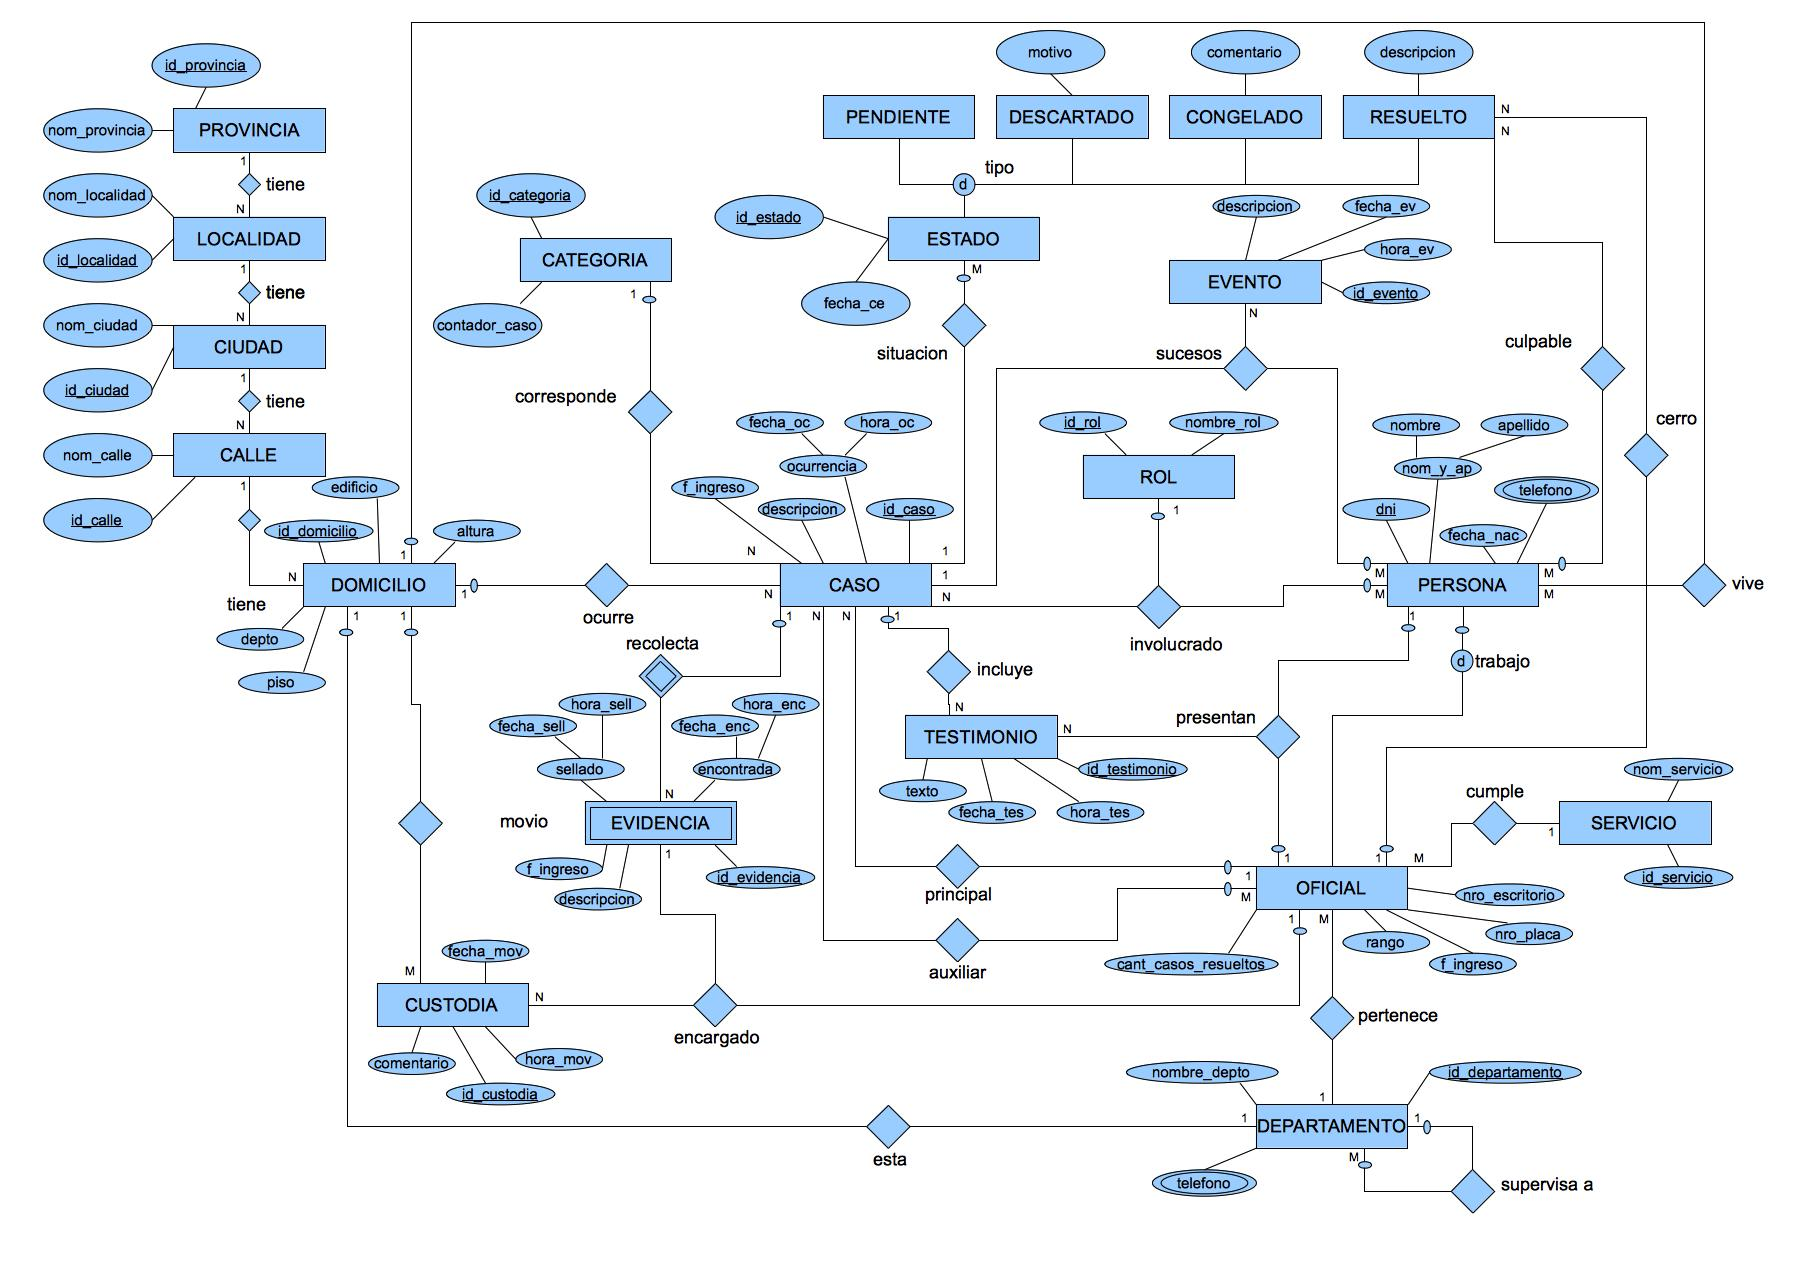
\includegraphics[angle=90, width=\linewidth]{figuras/DER_Final.jpg}
  \caption{Modelo Entidad Relación.}
  \label{fig:MER}
\end{figure}

\subsection{Restricciones adicionales}

\begin{itemize}
\item La fecha de ingreso de un caso debe ser posterior a la fecha de ocurrencia.

\item La fecha de ingreso de la evidencia debe ser posterior a la fecha de recolección.

\item La fecha de recolección de evidencia debe ser posterior a la fecha de ingreso del caso correspondiente.

\item La fecha de ocurrencia de un evento debe ser anterior a la fecha de ingreso del caso correspondiente.

\item Si se tiene una tupla $\langle c,o\rangle$ en principal, entonces no puede estar la misma tupla en auxiliar o viceversa.

\item Dada una tupla $\langle p,r \rangle$ en culpable, $\langle c,e \rangle$ en situación y $e.id\_estado$ $=$ $r.id\_estado$, entonces tiene que existir una tupla $\langle c,p,rol \rangle$ en involucrado.

\item Dada una tupla $\langle c,evento,p \rangle$ en sucesos debe existir la tupla $\langle c,p,rol \rangle$ en involucrado.

\item Dada una tupla $\langle c,p,rol \rangle$ en involucrado, si p además es un oficial, dicho oficial no puede estar relacionado con el caso c a través de principal o auxiliar.

\item Dada una tupla $\langle t,o,p \rangle$ en presentan, $o.dni \neq p.dni$

\item Dada la tupla $\langle o,r \rangle$ en cerro, debe existir una tupla $\langle c,o \rangle$ en principal o en auxiliar tal que $c.id\_caso$ $=$ $r.id\_caso$.
\end{itemize}


\newpage
\section{Modelo Relacional}

\par
\noindent \textbf{Provincia}(\underline{id\_provincia}, nom\_provincia) \\
\textbf{Localidad}(\underline{id\_localidad}, nom\_localidad, \dashuline{id\_provincia})\\
\textbf{Ciudad}(\underline{id\_ciudad}, nom\_ciudad, \dashuline{id\_localidad})\\
\textbf{Calle}(\underline{id\_calle}, nom\_calle, \dashuline{id\_ciudad})\\
\textbf{Domicilio}(\underline{id\_domicilio}, edificio, altura, depto, piso, \dashuline{id\_calle})\\
\textbf{Involucrado}(\underline{\dashuline{id\_caso}, \dashuline{dni}}, rol) (*)\\
\textbf{Resuelto}(\underline{\dashuline{id\_estado}}, descripción, \dashuline{dni})\\
\textbf{Culpable}(\underline{\dashuline{id\_estado}, \dashuline{dni}})\\
\textbf{Caso}(\underline{id\_caso}, categoría, f\_ingreso, descripción, fecha\_oc, hora\_oc, \dashuline{id\_domicilio}, \dashuline{dni})\\
\textbf{Testimonio}(\underline{id\_testimonio}, hora\_tes, fecha\_tes, texto, \dashuline{id\_caso})\\
\textbf{Pesona}(\underline{dni}, nombre, apellido, fecha\_nac, \dashuline{id\_domicilio})\\
\textbf{Oficial}(\underline{\dashuline{dni}}, rango, f\_ingreso, nro\_placa, nro\_escritorio, \dashuline{id\_servicio}, \dashuline{id\_departaento})\\
\textbf{Custodia}(\underline{id\_custodia}, comentario, hora\_mov, \dashuline{id\_domicilio})\\
\textbf{Evento}(\underline{id\_evento}, descripción, fecha\_ev, hora\_ev)\\
\textbf{Sucesos}(\underline{\dashuline{dni}, \dashuline{id\_evento}}, \dashuline{id\_caso})\\
\textbf{Evidencia}(\underline{\dashuline{id\_caso}, id\_evidencia}, fecha\_sell, hora\_sell, fecha\_enc, hora\_enc, f\_ingreso,descripción))\\
\textbf{Presentan}(\underline{\dashuline{id\_testimonio}, \dashuline{dni}}, \dashuline{dni})\\
\textbf{Encargado}(\underline{\dashuline{id\_custodia}, \dashuline{id\_evidencia}}, \dashuline{dni})\\
\textbf{Servicio}(\underline{id\_servicio}, nom\_servicio)\\
\textbf{Auxiliar}(\underline{\dashuline{dni}, \dashuline{id\_caso}})\\
\textbf{Departamento}(\underline{id\_departamento}, \dashuline{id\_departamento\_supervisor}, \dashuline{id\_domicilio})\\
\textbf{Telefono}(\underline{\dashuline{id\_departamento}}, teléfono)\\
\textbf{Telefono\_persona}(\underline{\dashuline{dni}}, teléfono)\\
\textbf{Situacion}(\underline{fecha\_ce, \dashuline{id\_estado}, \dashuline{id\_caso}})\\
\textbf{Pendiente}(\underline{\dashuline{id\_estado}})\\
\textbf{Descartado}(\underline{\dashuline{id\_estado}}, motivo)\\
\textbf{Congelado}(\underline{\dashuline{id\_estado}}, comentario)\\
\textbf{Estado}(\underline{id\_estado})\\

%- La relación involucrado es binaria N:M, sin atributo identificatorio, no dice cómo hacerlo en el apunte. Supongo que se hace así \\
%- Teléfono aparece como atributo multivaluado 2 veces, le cambio el nombre a uno para que no haya dos tablas distintas con el mismo nombre \\


\newpage
\section{Diseño Físico}


\newpage
\section{Códigos de Consultas}


\newpage
\section{Conclusiones}


\end{document}
